\documentclass[a4, 12pt]{article}
\usepackage[a4paper,top=1.3cm,bottom=2cm,left=1.5cm,right=1.5cm,marginparwidth=0.75cm]{geometry}
\usepackage{setspace}
\usepackage{cmap}
\usepackage{mathtext}
\usepackage[utf8]{inputenc}
\usepackage[english,russian]{babel}
\usepackage[T2A]{fontenc}
\usepackage{multirow}
\usepackage{graphicx}
\usepackage{wrapfig}
\usepackage{tabularx}
\usepackage{float}
\usepackage{longtable}
\usepackage{hyperref}
\hypersetup{colorlinks=true,urlcolor=blue}
\usepackage[rgb]{xcolor}
\usepackage{amsmath,amsfonts,amssymb,amsthm,mathtools}
\usepackage{icomma}
\mathtoolsset{showonlyrefs=true}
\usepackage{euscript}
\usepackage{mathrsfs}



\title{Маятник Фуко. Измерение угловой скорости вращения Земли.}
\author{Дудаков Семён, группа Б01-303}
\date{}

\begin{document}
	\maketitle
\newpage
\section{Введение}
Опыты по отклонению к востоку свободно падающих тел в принципе могли бы служить экспериментальным доказательство неинерциальности земной системы отсчета. Однако постановка таких опытов затруднительна, а их точность невелика. Для этой цели более подходящим является маятник Фуко. Он представляет собой массивный шар, подвешенный на очень длинной нити и совершающий малые колебания около положения равновесия. Отклоним маятник из положения равновесия, а затем представим его самому себе. Если бы Земля была инерциальной системой отсчёта, то на маятник действовали бы только "настоящие силы": сила тяжести и сила натяжение нити(силами трения и сопротивления воздуха пренебрегаем). Обе эти силы лежат в вертикальной плоскости. Поэтому если маятнику не сообщён толчок в боковом направлении, то он всё время будет колебаться в одной и той же вертикальной плоскости, неподвижной относительно Земли. Опыты показали, что это не так: плоскость качаний маятника в земной системе отсчёта медленно поворачивается вокруг вертикали рассматриваемого места и притом в том же направлении, в каком совершают суточное вращение Солнце и звезды на небесной сфере. Это доказывает, что земная система не является инерциальной
\section{Теория} 
Уравнение относительного движения материальной точки в неинерциальной системе отсчета:
\begin{equation*}
    m\mathbf{a}=\mathbf{F}-m\mathbf{\dot V_0}-m[\boldsymbol{\dot \omega_0}\mathbf{r}]+2m[\mathbf{v}\boldsymbol{\omega}]+m\omega^2\mathbf{r_\perp}
\end{equation*}
Уравнение относительного движения материальной точки в гравитационном поле Земли с учетом ее вращения:
\begin{equation*}
    m\mathbf{a}=(\mathbf{F_3} + m\omega^2\mathbf{r_\perp})+2m[\mathbf{v}\boldsymbol{\omega}]+\mathbf{F}
\end{equation*}
Пропали компоненты $m[\boldsymbol{\dot \omega_0}\mathbf{r}]$ и $m\mathbf{\dot V_0}$, так как Земля вращается практически равномерно.
Векторная сумма $(\mathbf{F_3} + m\omega^2\mathbf{r_\perp})$ пропорциональна массе точки $m$. Обозначим её $m\mathbf{g}$.\\
Итого получим:
\begin{equation*}
    m\mathbf{a}=m\mathbf{g}+2m[\mathbf{v}\boldsymbol{\omega}]+\mathbf{F}
\end{equation*}
\section{Исследование движения}
Рассмотрим малые колебания математического маятника с учётом силы Кориолиса.\\
Пусть маятник находится в точке земли с широтой $\alpha$. Разложим вектор угловой скорости на две составляющие: вертикальную $\boldsymbol{\omega_\text{в}}$ и горизонтальную $\boldsymbol{\omega__\text{г}}$. Горизонтальную в свою очередь разложим на две составляющие: $\boldsymbol{\omega_\parallel}$ и $\boldsymbol{\omega_\perp}$, из которых $\boldsymbol{\omega_\parallel}$ лежит в плоскости качаний маятника, а $\boldsymbol{\omega_\perp}$ к ней перпендикулярна.
\begin{figure}[H]
    \centering
    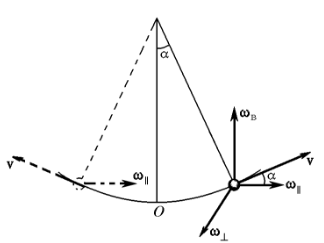
\includegraphics[scale = 0.7]{фуко.png}
    \caption{}
\end{figure}
Таким образом получим следующее уравнение движения:
\begin{equation*}
    m\mathbf{a}=m\mathbf{g}+2m[\mathbf{v}\boldsymbol{\omega}]+2m[\mathbf{v}\boldsymbol{\omega_\textbf{в}}]+2m[\mathbf{v}\boldsymbol{\omega_\perp}]+2m[\mathbf{v}\boldsymbol{\omega_\parallel}]+\mathbf{F}
\end{equation*}
Составлющая силы Кориолиса $2m[\mathbf{v}\boldsymbol{\omega_\perp}]$ направлена вдоль нити маятника. Она меняет натяжение нити, но на положение плоскости качаний влияния не оказывает, поэтому ей можно пренебречь.\\
Вторая составляющая силы Кориолиса $2m[\mathbf{v}\boldsymbol{\omega_\textbf{в}}]$ в нашей задаче наиболее важна. Она перпендикулярна к плоскости качаний маятника и вызывает вращение этой плоскости.\\
Третья составляющая $2m[\mathbf{v}\boldsymbol{\omega_\parallel}]$ тоже перпендикулярна к плоскости качания маятник, а потому она также оказывает влияние на вращение этой плоскости. Однако при рассматриваемых нами малых колебаниях её величина пренебрежимо мала.\\
В итоге уравнение движения маятника Фуко имеет вид:
\begin{equation*}
    m\mathbf{a}=m\mathbf{g}+2m[\mathbf{v}\boldsymbol{\omega_\textbf{в}}]+\mathbf{F}
\end{equation*}
При $\omega_\textbf{в}=0$ получаются обычные гармонические колебания маятника. Мы видим, что влияние силы Кориолиса приводит к вращению всей картины с угловой скоростью $\Omega_z$, где $\omega_\textbf{в}$=$\omega sin\alpha$.\\
\begin{figure}[H]
    \centering
    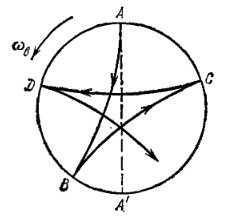
\includegraphics[scale = 0.7]{traek1.png}
    \caption{}
\end{figure}
\newpage
\begin{figure}
\centering
\begin{subfigure}{\textwidth}
  \centering
  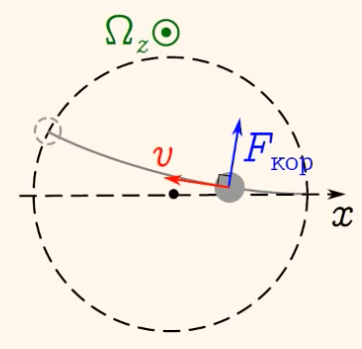
\includegraphics[width=.4\linewidth]{1f.png}
  \label{fig:sub1}
\end{subfigure}%
\begin{subfigure}{\textwidth}
  \centering
  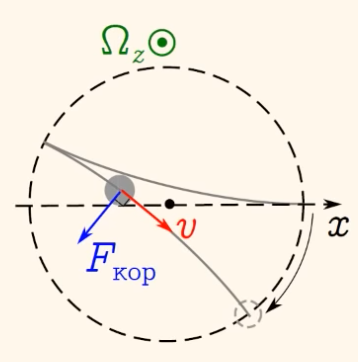
\includegraphics[width=.4\linewidth]{2f.png}
  \label{fig:sub2}
\end{subfigure}
\label{fig:test}
\end{figure}
\section{Вычисление угловой скорости вращения Земли}
Выше была приведена формула:
\begin{equation}
    \Omega_z = \Omega sin\lambda_0, \text{где } \lambda_0 - \text{широта}
\end{equation}
Откуда используя формулу для вычисления угловой скорости через период $(\omega=\frac{2\pi}{T})$, получим:
\begin{equation}
    \frac{2\pi}{\tau}=\frac{2\pi}{T}sin\lambda_0
\end{equation}
\begin{equation}
    T=\tau sin\lambda_0
\end{equation}
где $T$-период обращения Земли вокруг собственной оси, $\tau$-период обращения плоскости маятника Фуко\\
Таким образом, приняв широту Москвы $\lambda_0=55.733^\circ$, период обращения плоскости маятника Фуко на широте Москвы $\tau=28\text{ч }57\text{мин }41\text{с}$, вычислим период обращения Земли вокруг собственной оси, получим:
\begin{equation}
    T=23\text{ часа }56\text{ минут }3\text{ секунды}
\end{equation}
Теперь по формуле вычисления угловой скорости окончательно получаем:
\begin{equation}
    \omega=0.2624\text{ радиан/час }=15.04\text{ градусов/час}
\end{equation}
\section{Заключение}
В ходе проделанной работы было подробно изучено движение маятника Фуко, рассмотрена его траектория, доказана неинерциальность системы отсчета, связанной с Землёй, а именно доказано её вращение, а также была вычислена угловая скорость вращения Земли вокруг собственной оси.
\section{Список использованной литературы}
\begin{enumerate}
    \item Д.В. Сивухин, Общий курс физики, Том1 - Механика
    \item Л.Д. Ландау и Е.М. Лифшиц, Теоретическая физика, Том1 - Механика
    \item В.И. Арнольд, Математические методы классической механики
\end{enumerate}
\end{document}
